\subsection{Control to voltage}
\label{subsec:control_to_voltage}

As said in the previous section of mathematical modeling, we need to identify the relation between the control signal and the effective voltage applied to the coils.
The control unit provided by \texttt{Inteco} it's programmed to receive a PWM duty cycle as input and to convert it into a voltage that is applied to the coils.
In order to identify this relation, we simply apply many duty cycles to the control unit and measure the corresponding voltage applied to the coils using a multimeter.

The output of this test is a series of points that can be fitted to a linear model having an initial black zone where the control action is not effective on the voltage applied to the coils.
In Figure \ref{fig:control_to_voltage} we can observe both the measured points, the linear fitting and the effective voltage applied considering the black zone.

\begin{figure}[H]
    \centering
    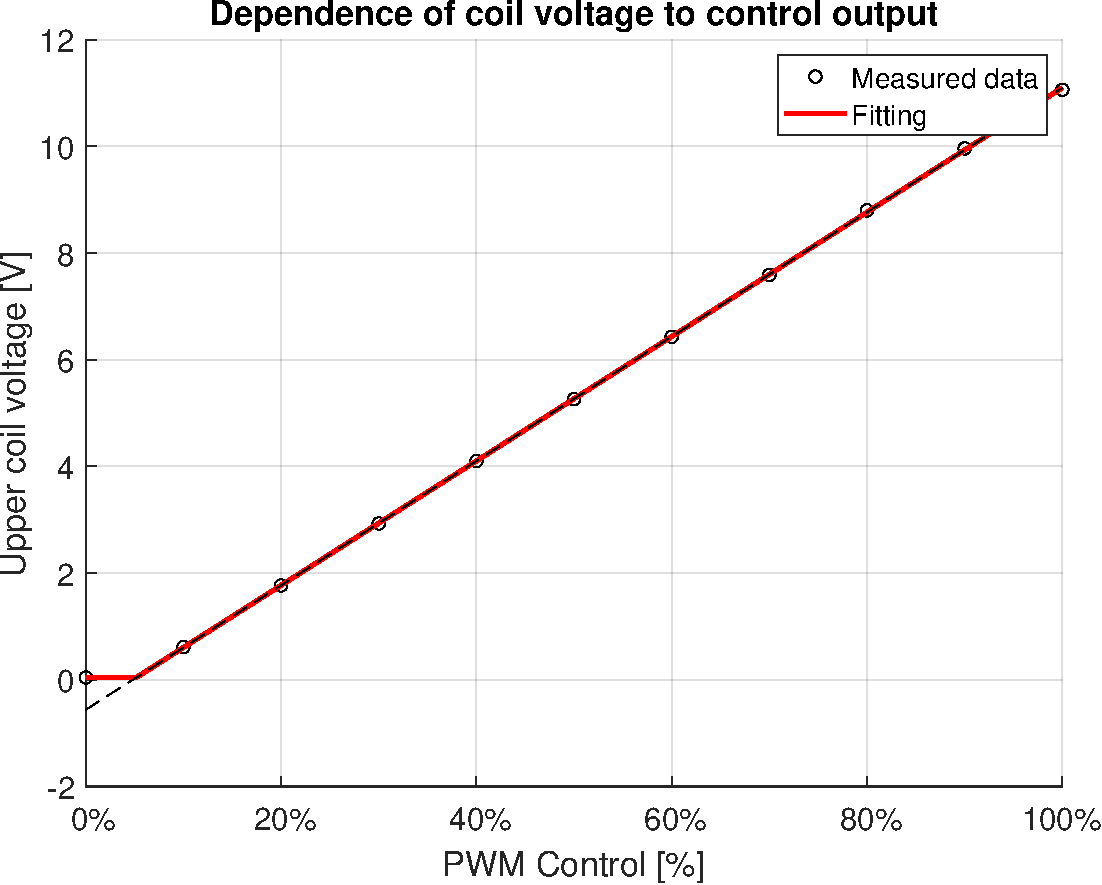
\includegraphics[width=0.6\textwidth]{img/MATLAB/identification/control_to_voltage.pdf}
    \caption{Control to voltage identification}
    \label{fig:control_to_voltage}
\end{figure}

As we can see, the linear model for the relation $V_* = f(U) = f(\text{PWM})$ is a good approximation outside the initial black zone control.
Because of this, we can consider the following control to voltage relation:

\begin{equation}
    V_* = \begin{cases}
        V_{*min}    & \text{if } U < U_{min}    \\
        k_* U + c_* & \text{if } U \geq U_{min}
    \end{cases}
\end{equation}

Where $V_{*min}$ is the minimum voltage applied to the coils when the control signal is zero, $u_{min}$ is the minimum control signal that is effective on the voltage applied to the coils, $k_*$ is the slope of the linear model and $c_*$ is the offset of the linear model.

The values of the parameters are shown in Table \ref{tab:control_to_voltage_parameters}.

\begin{table}[H]

    \centering
    \begin{tabular}{|c|c|c|}
        \hline
        \textbf{Parameter} & \textbf{Value}            & \textbf{Units} \\
        \hline
        $V_{*min}$         & $4.300000 \cdot 10^{-2}$  & $V$            \\
        $U_{min}$          & $5.179276$                & $\%$           \\
        $k_*$              & $1.165800 \cdot 10^{1}$   & $V/\%$         \\
        $c_*$              & $-5.608000 \cdot 10^{-1}$ & $V$            \\
        \hline
    \end{tabular}

    \caption{Control to voltage identification parameters}
    \label{tab:control_to_voltage_parameters}

\end{table}